\section{Consuntivazione}

\subsection{Attività svolte}

\begin{table}[ht]
    \begin{tabularx}{\textwidth}{X l l}
        
        \rowcolor{gray!30} \textbf{Attività} & \textbf{Stato} & \textbf{Ruolo}\\
        
        \hline
        verificata stesura processi primari avvenuta nell'iterazione precedente & completato & Amministratore\\
        svolte requisiti burocratici & completato & Responsabile\\
        \end{tabularx}
    \caption{Lista delle attività svolte durante lo sprint}
\end{table}


\begin{table}[ht]
    \begin{tabularx}{\linewidth}{X|rrrrrrr}
    \rowcolor{gray!30}& Re & Amm & An & Pro & Prog & Ver & tot \\
    \hline
    Bonavigo Michele                        & 0,5 & 0 & 0 & 0 & 0 & 0  & 0,5 \\
    \rowcolor{gray!10}Casarotto Mattia      & 0 & 0 & 0 & 0 & 0 & 0 & 0 \\
    Massarenti Alessandro                   & 0,7 & 0,1 & 0 & 0 & 0 & 0,4  & 1,2 \\
    \rowcolor{gray!10}Peron Samuel          & 0 & 0 & 0 & 0 & 0 & 0 & 0 \\
    Pierobon Luca                           & 0 & 0 & 0 & 0 & 0 & 0,3 & 0,3 \\
    \rowcolor{gray!10}Romano Davide         & 0 & 0 & 0 & 0 & 0 & 0 & 0 \\
    Zarantonello Giorgio                    & 0 & 0 & 0 & 0 & 0 & 0 & 0 \\
    \hline                                  & 1,2 & 0,1 & 0 & 0 & 0 & 0,7 & \\ 
    \end{tabularx}
    \caption{\label{ruoli-persone}Spartizione dei ruoli e ore svolte durante lo sprint}
\end{table}

\begin{center}
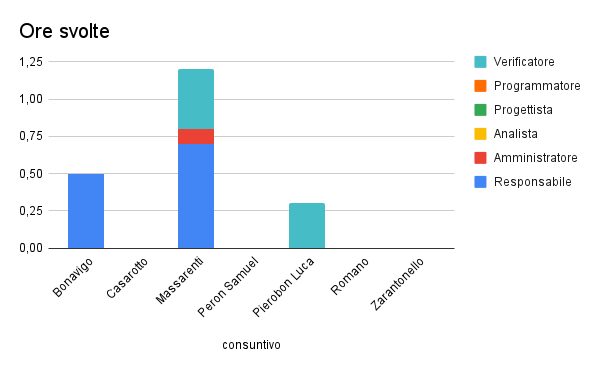
\includegraphics[width=12cm]{img/ore-svolte.png}
\end{center}

\begin{table}[ht]
    \begin{tabularx}{\linewidth}{X|l|l}
    \rowcolor{gray!30}& Ore & Costo \\
    \hline
    
    Responsabile & 1,2 & € 36,00 \\
    \rowcolor{gray!10}Amministratore & 0,1 & € 2,00 \\
    Analista & 0 & € 0,00 \\
    \rowcolor{gray!10}Progettista & 0 & € 0,00 \\
    Programmatore & 0 & € 0,00 \\
    \rowcolor{gray!10}Verificatore & 0,7 &€ 10,50 \\
    totale & 2 & € 48,50 \\
    \end{tabularx}
    \caption{\label{costi-ruolo}Spartizione dei ruoli e ore svolte durante lo sprint}
\end{table}


Avendo quindi consumato €48,50\footnote{Si veda tabella \ref{costi-ruolo}} del budget durante questo sprint, rimangono ancora a disposizione € 11787,50 per gli sprint seguenti.

\subsection{Trend e riflessioni}

\begin{figure}[ht]
    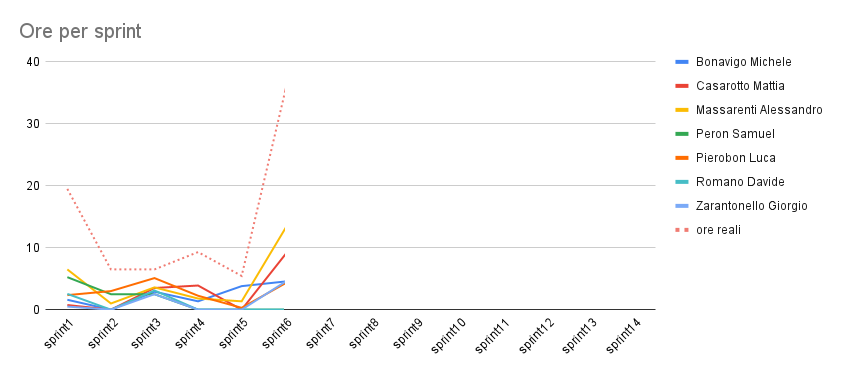
\includegraphics[width=\linewidth]{img/andamento.png}
    \caption{Andamento ore utilizzate nei vari sprint}\label{img:andamento}
\end{figure}

Come descritto nella sezione \ref{preventivo} relativa al preventivo, questo sprint è molto rallentato per via degli esami in corso. Il gruppo non è soddisfatto e prevede di impegnarsi con più decisione negli sprint successivi.

\subsection{Difficoltà e problemi di sprint}

Alcune questioni sono risultate\footnote{alcune questioni purtroppo non sono state risolte rispetto allo sprint precedente} durante questo sprint:

\begin{itemize}
    \item il gruppo si è concentrato molto sugli esami, mettendo in primo piano gli obiettivi a breve termine;
    \item il proponente non ha ancora definito il supporto hardware per i lampioni a cui dovremo far fede.
\end{itemize}

In retrospettiva il gruppo ha iniziato ad elaborare come la scelta di mettere in coda questa attività non sia costruttiva.
Il feedback al diario di bordo DRO\_20230129 ci ha aiutato a ragionare e a comprendere meglio la questione.

Queste difficoltà verranno inoltre discusse in sede di preparazione del prossimo sprint.
